% !TEX root = ./CA_solution.tex

\section*{5장 - 연습문제 풀이}

\subsection*{연습문제 \ref{ex-5-1}}

\begin{itemize}
\item[(1)] $(x,y)\in \mathbb R^2\setminus\{(0,0)\}$에 대하여
\begin{align*}
\dfrac{\partial u}{\partial x} &= \dfrac1{x^2+y^2} \cdot 2x = \dfrac{2x}{x^2+y^2} \\
\dfrac{\partial^2 u}{\partial x^2} &= \dfrac2{x^2+y^2} - \dfrac{2x}{(x^2+y^2)^2} \cdot (2x) 
= \dfrac{2y^2+2x^2-4x^2}{(x^2+y^2)^2} = \dfrac{2(y^2-x^2)}{(x^2+y^2)^2}.
\end{align*}
$x$, $y$에 대한 대칭식임을 이용하면
\[
\dfrac{\partial u}{\partial y}  = \dfrac{2y}{x^2+y^2}, \quad
\dfrac{\partial^2 u}{\partial y^2} = \dfrac{2(x^2-y^2)}{(x^2+y^2)^2}.
\]
따라서,
\[
\dfrac{\partial^2 u}{\partial x^2} + \dfrac{\partial^2 u}{\partial y^2}
= \dfrac{2(y^2-x^2)}{(x^2+y^2)^2} + \dfrac{2(x^2-y^2)}{(x^2+y^2)^2} = 0.
\]
$\mathbb R^2\setminus\{(0,0)\}$에서
$u\in C^2$이고 $\Delta u=0$이므로, $u$는 조화함수이다.
\item[(2)] 
$(x,y) \in \mathbb R^2$에 대하여
\begin{align*}
\dfrac{\partial u}{\partial x} &= e^x\sin y, \ \dfrac{\partial^2 u}{\partial x^2} = e^x\sin y, \\
\dfrac{\partial u}{\partial y} &= e^x\cos y, \ \dfrac{\partial^2 u}{\partial y^2} = e^x(-\sin y).
\end{align*}
따라서, 
$\dfrac{\partial^2 u}{\partial x^2} + \dfrac{\partial^2 u}{\partial y^2}
= e^x\sin y + e^x(-\sin y) = 0$.
$\mathbb R^2$에서
$u\in C^2$이고 $\Delta u=0$이므로, $u$는 조화함수이다.
\end{itemize}

\subsection*{연습문제 \ref{ex-5-2}}

$U$에 정의된 실변수 함수의 점별연산에 대한 공간 $V$를 생각하자.
$V$는 벡터공간이 됨을 알고 있다.
$\Har(U)$가 점별연산에 대하여 $V$의 부분공간을 이룬다는 것을 증명하자.
\begin{itemize}
\item[(S1)]
$U$의 모든 점에서 $0$을 대응시키는 상수함수 $\bs 0$가 $\Har(U)$에 속한다.
\[
\dfrac{\partial^2 \bs 0}{\partial x^2} + \dfrac{\partial^2 \bs 0}{\partial y^2} = 0+0=0.
\]
\item[(S2)] $u,v\in \Har(U)$라고 하면,
\begin{align*}
\dfrac{\partial^2 (u+v)}{\partial x^2} + \dfrac{\partial^2 (u+v)}{\partial y^2}
&= \dfrac{\partial^2 u}{\partial x^2} + \dfrac{\partial^2 v}{\partial x^2}
+ \dfrac{\partial^2 u}{\partial y^2}+ \dfrac{\partial^2 v}{\partial y^2} \\ 
&= \left(\dfrac{\partial^2 u}{\partial x^2} + \dfrac{\partial^2 u}{\partial y^2} \right)
+ \left( \dfrac{\partial^2 v}{\partial x^2} + \dfrac{\partial^2 v}{\partial y^2} \right) \\
&= 0+0=0.
\end{align*}
\item[(S3)] $\alpha\in\mathbb R$이고, $u\in\Har(U)$이면,
\begin{align*}
\dfrac{\partial^2 (\alpha\cdot u)}{\partial x^2} + \dfrac{\partial^2 (\alpha\cdot u)}{\partial y^2}
&= \alpha\cdot \dfrac{\partial^2 u}{\partial x^2} 
+ \alpha \cdot \dfrac{\partial^2 u}{\partial y^2} \\
&= \alpha \left( \dfrac{\partial^2 u}{\partial x^2} + \dfrac{\partial^2 u}{\partial y^2} \right)
= \alpha\cdot 0 = 0.
\end{align*}
이상에서 $\Har(U)$는 점별연산에 대하여 실 벡터공간이 된다.
\end{itemize}

\subsection*{연습문제 \ref{ex-5-3}}


\begin{figure}[h!]
\begin{center}
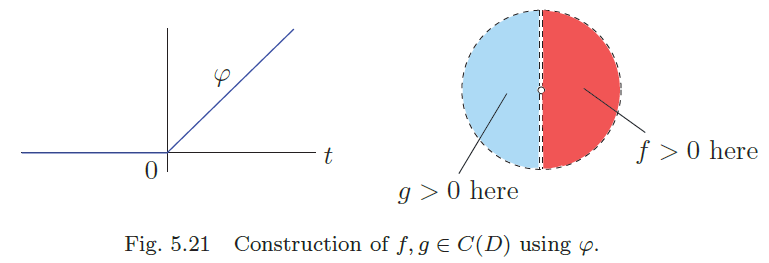
\includegraphics[width=0.8\textwidth]{./figs/fig-5-21}
\end{center}
\caption{$\varphi$를 이용한 연속함수 $f,g\in C(D)$ 설정
}
\label{fig-5-21}
\end{figure}






